\label{fs-acker-preliminaries}

First, in this section, we formalize a stream processing engine based on Chandy-Lamport definition of a distributed system. Then we define the substream management problem based on the notions from the proposed model. Finally, we discuss a state-of-the-art substream management technique called punctuations.

\begin{table}[!b]
    \caption{Notations used throughout the paper}
    \footnotesize
    \begin{tabular}{l|p{5cm}}
        \hline
        $p$ & Process (node in a physical execution graph) \\ 
        \hline
        $I_p$, $O_p$ & input and output channels of a process $p$ \\ 
        \hline
        $func_p(U, M)$ & User-defined operator run by process $p$. It receives current operator state $U$ and an incoming message $M$ \\ 
        \hline
        $\Pi$ & The set of all processes  \\
        \hline
        $K$ & Number of substreams  \\
        \hline
        $c$ & A network channel between processes  \\
        \hline
        $\mathcal{E}$ & The set of all network channels  \\
        \hline
        $s_p = U_p \cup B_p$ & State of the process $p$ consists of a mailbox $B_p$ and a state $U_p$ of $func_p$ \\
        \hline
        $mbc_{p}$ & Mailbox controller of a process $p$ \\
        \hline
        $e_{p}$ & Event of a process $p$ \\
        \hline
        $Pred(e)$ & Propositional formula defined on events \\
        \hline
        $pred(M)$ & Propositional formula defined on messages\\
        \hline
        $t(M)$ & Coarse time label \\
    \end{tabular}
    \label{notations}
\end{table}

\subsection{Processing model}
\label{fs-acker-processing-model}

Typically, distributed stream processing engines are shared-nothing runtimes that continuously ingest input elements, transform them according to a logical dataflow graph, and deliver output elements. The logical dataflow graph consists of user-defined operators. Operators are functions of a single input data element that produce a number of output data elements. Operators can be stateless or stateful: output elements may depend on the current state. A logical graph is mapped to a physical, distributed graph on deployment. Commonly, a single logical operator can be deployed on multiple computational nodes. Further, we denote physical instances of logical operators as {\em processes}.

A deployed physical graph is a distributed system and could be described in terms of the Chandy-Lamport model~\cite{Chandy:1985:DSD:214451.214456, carbone2018scalable}. In this model, the authors introduce \textit{events} that allow observing a state of the entire system. This approach allows defining system-wide guarantees: in the original paper, it is used to introduce the notion of {\em consistent state}, we use this approach for the definition of a substream management problem.

Following the notation from~\cite{Chandy:1985:DSD:214451.214456, carbone2018scalable}, the distributed system is observed with events. Each event is a tuple of 5 elements $e = (p, s, s', c, M)$, where $p$ is one of the deployed processes, $s$ and $s'$ are state of the process before and after processing, $c$ is one of network FIFO channels that connect processes, and $M$ is a message generated during processing. The generated event $M$ comes to a channel state $C$ until the destination process receives it. Processes and channels form a physical graph of the system $G=\{\Pi,\mathcal{E}\}$. We denote all input channels as $I_p$ and output channels as $O_p$.

In a stream processing engine, we need to specify a process $p$ to reflect the nature of SPE. In our model we split a process into two separate blocks: {\em business logic handler} (BLH), and {\em mailbox controller} (MBC). The first block encapsulates a user-defined operator. In this model user-defined operator does not directly communicate with other processes in the system. Instead of this, it receives and generates {\em messages} -- data elements that are tagged by their source and destination. Further delivery of these messages along the communication channels is then handled by a mailbox controller that preserves the order of message generation. Figure~\ref{fig:spe_process} illustrates the scheme of a process. This system layout is not new, and it is widely used in practice (Akka, YDB, Millwheel, etc.).

\begin{figure}[t]
  \centering
  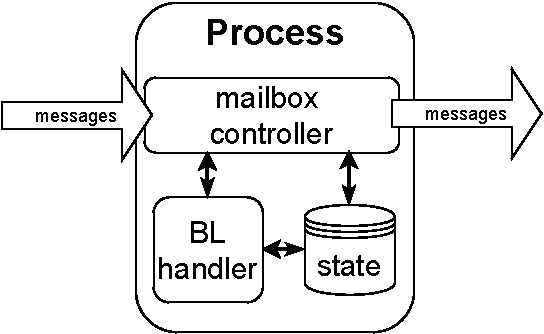
\includegraphics[width=0.3\textwidth]{pics/process-scheme.pdf}
  \caption{Structure of the SPE process}
  \label{fig:spe_process}
\end{figure}

More formally, when a process receives a message, it is handled by the mailbox controller that puts this message into a special segment of the process state ({\em mailbox} $B_p$). The business logic handler gets a message provided by MBC and triggers a user-defined operator. The user-defined operator processes the data element that the message contains and generates an arbitrary number of outgoing messages. BLH puts generated messages back to a mailbox. MBC sends outgoing messages along communication channels to destination processes. All mailbox controller operations respect the order of messages in the mailbox. If a user-defined operator has a state $U_p$, the joined process state will consist of the mailbox and this state $s=U_p \cup B_p$. In the Chandy-Lamport paradigm this algorithm produces the following events within a process:
\begin{itemize}
    \item Communication events: $\langle recv, p, M\rangle$, $\langle send, p, M \rangle$ -- these events are handled by mailbox controller
    \item Processing of an incoming message $\langle proc, p, M, M' \rangle$
\end{itemize}

Lets translate these events into 5-tuple language. Communication events move a message between communication channel and mailbox section of the state:
\begin{eqnarray}
\langle recv, p, M\rangle = (p, s_p, s'_p = U_p \cup \left(B_p \cup \{M\}\right), c_{qp}, M) \\
\langle send, p, M \rangle = (p, s_p, s'_p = U_p \cup \left(B_p\setminus\{M\}\right), c_{p, dst(M)}, M)
\end{eqnarray}

Note that we need to be able to get a destination process directly from the message $dst(M)$. This function translates a destination element from logical dataflow graph nodes, used in user-defined code, to physical communication channels between processes. A practical case of this abstraction is a sharding scheme for some key: user-defined procedure emits event for some key, and a system is responsible for finding a proper physical channel to deliver this message.

Incoming message processing does not influence the communication channels and only ingest results of a message processing $(U', M') = func_p(U, M)$:
\begin{equation}
    \langle proc, p, M, M' \rangle = (p, s_p, s'_p = U'_p \cup \left(B_p \setminus \{M\} \cup M' \right) , \emptyset, \emptyset)
\end{equation}

Note that in this case, $M'$ may contain more than one message. Following the Chandy-Lamport model, we assume processes are single-threaded, so within the specific process $p$, all events are ordered by a local causal order relation $<_p$: $e^{0}_p,e^{1}_p,\ldots,e^{i}_p,\ldots$. Please note that each process has its own local causal order relation, so we do not assume any total order among events from different processes. This model is indeed practical, e.g., implemented in actor-based systems.

% Substream system events will be defined latter in the description of a particular implementation. Note that all events within the same process $p$ are totally ordered by a local causal order relation $<_p$: $e^{0}_p,e^{1}_p,...,e^{i}_p,...$. 
% Atomicity of the events and their sequential nature allows a system to build guarantees for processing and state management.

\subsection{Substream management events}
\label{fs-acker-substream-events}
% The processing of unbounded data sequences sometimes is difficult, and it is easier to solve an unlimited stream of small tasks than a single task for an unlimited stream of data. We filter data elements with a condition to limit the scope of a task. The data elements that satisfy a condition form a {\em substream}. The practical examples of substreams are: ``clicks received in time window $w$'', or ``requests from user 0x0321da83'', etc.

\subsubsection{Substreams lifespan}

For each process, we want to get the first and the last element of a substream. The first one could be found naturally when it emerges, but verification that there will be no more events of a substream could be problematic. Strict substream termination guarantee consists of two parts: source must promise that no more messages from substream may emerge, and the system must ensure it contains no substream messages. The first task requires a contract with a particular data source and is thus out of scope for this paper, though it is discussed in relevant literature~\cite{awad2019adaptive}. Instead, we focus on the second task; this is challenging due to distributed nature of the system and the lack of a common message lifetime limit. This difficulty increases with the introduction of cycles into dataflow. Crucially, processes are not isolated from one another, and substream messages can move from one process to another. That is why we need to observe all in-flight messages in the system.

Formally, a substream can be defined via the propositional formula $Pred(e)$ for any system event. We have to use system events as they are ordered inside each process and can define a border of a substream. Sometimes it is more practical to induce this predicate to messages ($pred(M)$) involved in processing: $Pred(e) = (e = \langle proc, p, M, M'\rangle) \wedge pred(M)$.

In this paper we are interested in such $Pred(e)$, that has limited lifespan within a process and want to know when substream starts and terminates: $\forall p, \exists t_0^p, t_1^p: \exists e: e_{t_0^p} <_p e <_p e_{t_1^p}, Pred(e) \And \forall e': e_{t_1^p} <_p e', \neg Pred(e')$. Lets boil this formula down: for each process $p$ in the system there must be two event indices $t_0^p$ for substream start and $t_1^p$ for its termination, such that events satisfying $Pred$ must be between these indices. 

{\em Substream management problem} is to define a special mechanism that estimates substream bound for each process. In our system model, we need to define a system event that indicates the bound of a substream for a process. We call this termination event or end-of-substream event, this appropriate :
\begin{equation}
  \langle eoss, p, Pred \rangle = (p, B_p, B_p\cup eoss(Pred), \emptyset, \emptyset)  
\end{equation}

As we mentioned before, some problems require certain properties of the termination events. For example, the state pruning problem does not require any special properties, while for the state snapshotting problem, the substream management system should detect the exact substream bound. In the following sections, we formalize these properties. 

\subsubsection{Soft bound}

Many applications that apply substream management systems do not require any special properties of termination events. In this case, we denote the guarantee provided by such events as {\em soft bound}, because termination events indicate only the fact that the substream ended some time ago, and other input elements could be processed after that. More formally, we define the soft bound guarantee of the termination event (end-of-substream) $\langle eoss_{soft}, p, Pred\rangle$ as follows:

\begin{equation}
\forall e, e >_p \langle eoss_{soft}, p, Pred\rangle \Rightarrow \neg Pred(e)
\end{equation}

Figure~\ref{general_guarantees} illustrates this notion. Terms $a,b,c,d...$ denote ordered processing events of a process $p$. The substream ends after event $c$. Note that there are several other events between the end-of-substream and $c$. This is the property of a {\em soft bound} guarantee: if $\langle eoss_{soft}, p, Pred\rangle$ occurs, all subsequent elements do not satisfy the predicate, but it is not necessarily the exact substream ``border''.

\begin{figure}[t]
  \centering
  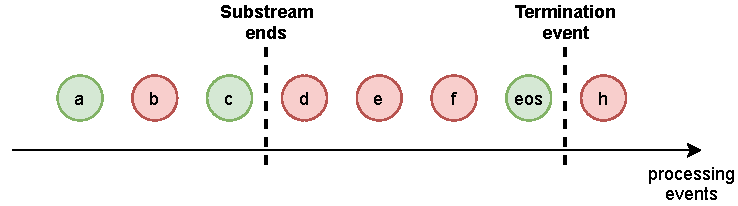
\includegraphics[width=0.50\textwidth]{pics/general-guarantee.pdf}
  \caption{Substream management: soft bound}
  \label{general_guarantees}
\end{figure}

\subsubsection{Firm bound}

The guarantee that any new event will not satisfy the predicate is sufficient for many real-life problems, e.g., SPE can initiate process state pruning on such events. However, some problems require a {\em firm bound}: guarantee that the substream ends {\em exactly} after the termination event. 

For example, epoch-based snapshotting protocol~\cite{2015arXiv150608603C, jacques2016consistent} relies on the notion of {\em epoch}. An epoch is a special substream that must be processed atomically. Therefore, the SPE requires the termination event for a given epoch to occur immediately after the last processing event for that epoch. Otherwise, the snapshot can be inconsistent, capturing elements from multiple epochs. To support such scenarios, the end-of-substream event $\langle eoss_{firm}, p, Pred\rangle$ should satisfy the following condition:

\begin{equation}\begin{array}{l}
\langle eoss_{firm}, p, Pred\rangle = \inf_{<_p} \langle eoss_{soft}, p, Pred\rangle
\end{array}\end{equation}

Unlike the soft bound, within the firm guarantee, the first element outside the substream $Pred$ must be ordered after the firm bound event in the process $p$. This position satisfies the first possible soft bound in the events ordering. Figure~\ref{strict_guarantees} illustrates the notion of the firm bound. As in the previous example, terms $a,b,c,d...$ denote ordered processing events of a process $p$. However, in this case, event $\langle eoss_{firm}, p, Pred\rangle$ occurs right after the substream terminates.

\begin{figure}[t]
  \centering
  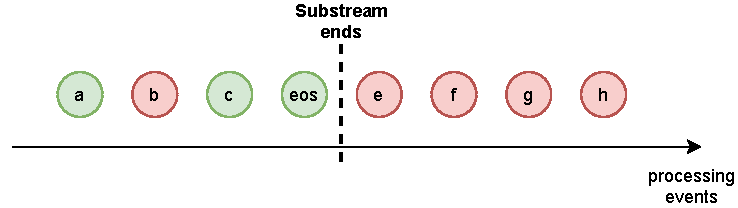
\includegraphics[width=0.50\textwidth]{pics/strict-guarantee.pdf}
  \caption{Substream management: firm bound}
  \label{strict_guarantees}
\end{figure}

\subsubsection{Consistent termination events order}
Some specific applications, including the mentioned earlier epoch-based snapshotting method and techniques for enforcing deterministic processing~\cite{we2018adbis} require an order of termination events to be synchronized with the order of substreams last elements processing. For example, if termination events are reordered, then snapshots for consecutive epochs can be inconsistent. Another example is deterministic join that also requires the defined order of termination events~\cite{gulisano2016scalejoin}.

\begin{figure}[htbp]
  \centering
  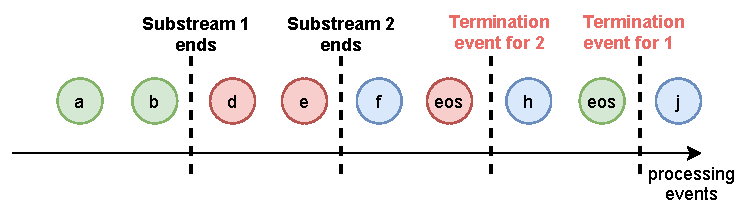
\includegraphics[width=0.50\textwidth]{pics/notifications-reordering.pdf}
  \caption{An example of termination events reordering}
  \label{notifications_reordering}
\end{figure}

Termination events reordering in case of the soft bound guarantee is illustrated in Figure~\ref{notifications_reordering}. Terms $a,b,c,d...$ denote ordered processing events of a process $p$. Although the substream containing events $a,b$ terminates earlier, the end-of-substream event for this substream occurs after the termination event for the substream containing events $d,e$. 

Let $e^{*}_1$ and $e^{*}_2$ be the last elements of substreams defined by predicates $Pred_1$ and $Pred_2$. Termination events $\langle eoss, p, Pred_1\rangle$ and $\langle eoss, p, Pred_2\rangle$ are {\em consistently ordered} iff:

\begin{equation}
e^{*}_1 >_p e^{*}_2 \Leftrightarrow \langle eoss, p, Pred_1\rangle >_p \langle eoss, p, Pred_2\rangle
\end{equation}

\subsubsection{Optimal traffic overhead}

A vital performance property of a substream management system is the amount of extra network traffic. Let $|\Pi|$ be a number of processes, and $K$ be a number of substreams. 

\begin{lemma}
The network overhead induced by a substream management system cannot be lower than $O(K|\Pi|)$. 
\end{lemma}
\begin{proof}
We assume one by one processing of substreams for them to be isolated (e.g. epochs). When a substream management system detects the termination of a substream, each stateful process should be informed about this. Hence, at least one network message (termination notification) must be received by each process for each substream.
\end{proof}

% Despite the simplicity of this lemma, it will be further used to determine how far a given substream management system is from the theoretical bound. We can also claim a solution is {\em optimal} as its extra traffic estimation is equal to the lower bound of the lemma.
% In the next sections, we demonstrate that it is possible to design a substream management system that achieves optimal network traffic overhead.

\subsection{Punctuations framework}
\label{fs-acker-punctuations}

To justify the usefulness of our model described above in Section~\ref{fs-acker-substream-events}, we show how our model can describe the most widely used by state-of-the-art SPEs substream management framework called {\em pucntuations}. We also prove certain properties which are inherent to any implementation of the punctuations framework. 

The main idea behind the punctuations framework is to inject special data elements $\mathcal{P}^{pred}$ into data stream one per substream. These elements, called punctuations, flow down the workflow as ordinary data elements. The injector promises that all elements after punctuations won't satisfy the predicate. Hence, the punctuation itself defines the ``border'' of a substream.

Figure~\ref{punctuations_scheme} illustrates the punctuations framework. Green elements indicate elements that belong to some substream, while red elements do not. As we can see, punctuations play the role of delimiter between the substream elements and all further items.

\begin{figure}[htbp]
  \centering
  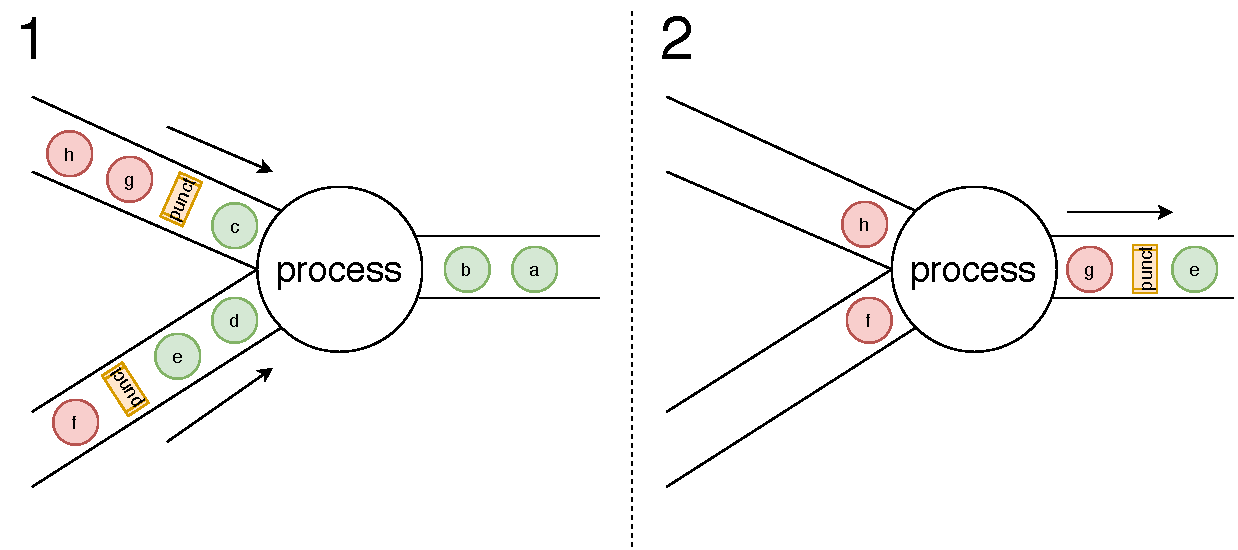
\includegraphics[width=0.40\textwidth]{pics/punctuations-scheme.pdf}
  \caption{Punctuations handling by a single process}
  \label{punctuations_scheme}
\end{figure}

Processes within SPE do not apply user-defined operators to punctuations. Instead, each process $p$ propagates punctuation messages $\mathcal{P}_{pq}^{pred}$ to all outgoing channels $c_{pq} \in O_p$  when it receives corresponding punctuations from all input channels $I_p$.

\begin{lemma}
Generating event by following rule make it a soft bound of a substream $pred$:
\begin{equation}
\forall q \in I_p, \exists \mathcal{P}^{pred}_{qp} \in B_p, \forall M\in B_p : \neg pred(M) \vee dst(M) \ne p
\end{equation}
\end{lemma}
% \begin{proof}
% Using the definition of the soft bound, we can use indirect proof. If there is a processing event from the substream that happens after the generated event, there is a message $M^*$ that generates this event. This message could emerge from two sources: from the mailbox of a process or from incoming channels. The mailbox does not contain such elements due to condition $pred(M) \wedge dst(M) = p$. Data sources guarantee that after a punctuation element, they will provide the system with no substream elements. This condition allows us to say that the data element entered the system before punctuation. Because of broadcasting on each step, punctuations cover all possible processing paths of a data element, including the processing path of the particular message $M^*$. This means that the punctuation message and data element from $M^*$ were reordered along the processing path, which contradicts with either mailbox controller order preservation or the FIFO nature of communication channels.
% \end{proof}

\begin{proof}
We can use indirect proof. Let $\langle proc, p, M^*, M' \rangle$ be a processing event that happens after the soft bound termination event but $pred(M^*)$. In other words, there is a message $M^*, pred(M^*)$ that arrived after all punctuations for the predicate $pred$ had been arrived. According to the definition of a distributed system from Section~\ref{fs-acker-processing-model}, message $M^*$ could emerge either from the mailbox of a process or from incoming channels. The emergence from the mailbox contradicts the condition of the termination event generation rule $\forall M\in B : \neg pred(M) \vee dst(M) \ne p$. On the other side, if element come from an incoming channel, we can track it's path through the system from a data source to the channel (processing path). Because of broadcasts on each step, watermarks travel all possible paths in the system including the path, that traveled the element. Along this path they were reordered. This could happen either during transmission, or during processing. The first hypothesis contradicts with the FIFO nature of communication channels. The second one is impossible due to definition of the processing model, that protects a processing order. We excluded all possible ways of getting event $M^*$ and have to reject initial hypothesis.
\end{proof}

To satisfy the firm bound guarantee, the mailbox controller should block processing of all incoming messages from a channel as soon as it receives punctuation from this channel. In~\cite{Carbone:2017:SMA:3137765.3137777} such behavior is called {\em watermark (punctuation) alignment}. Formally we can rewrite this requirement in terms of event ordering:

\begin{lemma}
A soft bound becomes firm if a process event order satisfy the following conditions:
\begin{equation}
  \forall e_1, e_2 = \langle recv, p, \mathcal{P}^{pred}_{q_{1,2}p} \rangle, \nexists e' = \langle proc, p, M_{q_1p}, M' \rangle, e_1 <_p e' <_p e_2
  \label{eq:firm_condition}
\end{equation}
\end{lemma}
\begin{proof}
Let us suppose that there is a message $M_{qp}$ of a next substream that was processed after the last element of the current substream, but before the generation of a bound event. This message either came from the channel $q$ before a punctuation from that channel generating a bound, or was processed before all channels delivers their punctuations. The first case could happen if $M_{qp}$ was reordered with the punctuation along the processing path and contradicts with FIFO processing logic (see previous proof for details). The second case is impossible because of processing limitations introduced by~\ref{eq:firm_condition}.
\end{proof}

The design of the punctuations framework implies two important properties:

\begin{enumerate}
    \item {\bf Lack of cyclic dataflows support.} Although there are techniques that extend punctuations for state snapshotting of iterative processing~\cite{Carbone:2017:SMA:3137765.3137777}, the termination of a general substream cannot be determined using punctuations framework if an execution graph contains cycles.
    \item {\bf Network traffic complexity quadratically depends on the number of processes.} As we demonstrated above, each process waits for punctuations from all incoming network channels delivers. It leads to high network traffic overhead if all processes are interconnected.
\end{enumerate}

\begin{lemma}
Punctuations framework cannot determine substream termination of an execution graph contains cycle.
\end{lemma}
\begin{proof}
If we have a cycle in the processing graph we can find a process that receives input from the latter steps of the cycle (back-link). This process will propagate a punctuation element when all incoming channels have received their punctuation elements. Due to cycle, for a back-link channel this punctuation element processing path contains the process itself (as a starting element of the cycle) and this means that to generate a punctuation we need it to be already generated. Contradiction.
\end{proof}

Despite the Lemma we just proved, some punctuation based systems report support of cyclic workflows. This is practically achieved with the limitation on the number of possible entrances into cycle by some $m$. With this limitation, we can roll out the cycle with repeating fragment of the cycle $m$ times. The first block is then connected to the input of the cycle, and the last element of the cycle to two elements: repetition entrance and the output of the cycle. Repetitions are organized the same way. From theoretical perspective this representation of the cycle is a DAG, that indeed could be served by punctuation mechanism.

\begin{lemma}
Network traffic complexity for this method is $O(K|\Pi|^2)$, where $|\Pi|$ is the number of processes and $K$ is the number of substreams if an SPE distributes the work among processes evenly.
\end{lemma}
\begin{proof}

Even the soft bound event requires receiving punctuations from all incoming network channels. If a distributed stream processing engine balances the work evenly among the processes, all processes are interconnected. Therefore, each active process should broadcast punctuations to all other processes. If we assume that all proccesses involved into processing of the elements that belong to predicate, the transmission complecsity of punctuation elements is $O(K|\Pi|^2)$. Therefore, if the number of existing substreams is $K$ then the network traffic complexity for the punctuations framework is $O(K|\Pi|^2)$ because each process should broadcast punctuations for each substream. 

\end{proof}

Note that the are several promising directions of improving the network traffic complexity for punctuations framework. Firstly, we can batch punctuations for several substreams. It can reduce network complexity to $O(\frac{K}{B}|\Pi|^2)$ where B is a batching frequency. On the other hand, such approach can increase the latency between the substream end and the termination event while keeping the quadratic dependency on the number of nodes.

Secondly, it is possible to attach punctuations to all regular input data elements. In this case, there can be no extra traffic in terms of messages at all. However, it makes the latency between the substream end and the termination event completely unpredictable because some network channels can be used rarely.

Both mentioned optimization ideas have important trade-offs and require deep theoretical and experimental research. Therefore, we do not consider mentioned optimization ideas in this work leaving them for the future work.